\documentclass{article}
\usepackage[utf8]{inputenc}
\usepackage[T1]{fontenc} 
\usepackage[slovene]{babel} 

\usepackage{enumitem} 
\usepackage{amsmath}
\usepackage{amsthm} 
\usepackage{amssymb}
\usepackage{lmodern}
\usepackage{amsfonts} 
\usepackage{mathtools}
\usepackage{graphicx}
\graphicspath{ {./images/} }

\DeclareMathOperator*{\argarg}{Arg}
\DeclareMathOperator*{\rere}{Re}
\begin{document}
\title{Schwarzov princip zrcaljenja za harmonične funkcije\\
    \Large Diplomska naloga
}
\author{
    Matej Novoselec\\
    Fakulteta za matematiko in fiziko\\
    Oddelek za matematiko\\
    Mentorica: Barbara Drinovec Drnovšek
}
\date{7.\ april 2022}


\theoremstyle{definition}
\newtheorem{defi}{Definicija}[section]
\theoremstyle{definition}
\newtheorem{op}[defi]{Opomba}
\newtheorem{trditev}{Trditev}[section]
\newtheorem{pro}{Problem}[section]
\newtheorem{lema}{Lema}[section]
\newtheorem{izrek}{Izrek}[section]
\newtheorem*{kons}{Konstrukcija}

%------------------------------------------------------------
\maketitle
\bibliography{.bib}
\bibliographystyle{siam}
\section{Uvod}

\section{Harmonične funkcije}
    \begin{defi}
        Funkcija $u(x_1, x_2, \dots, x_n)$ je \textbf{harmonična}, če velja
        $$
        \frac{\partial^2 u}{\partial x_1 ^ 2} +  \frac{\partial^2 u}{\partial x_2 ^ 2} + \dots + \frac{\partial^2 u}{\partial x_n ^ 2} = 0.
        $$
        Operatorju $\Delta  = \frac{\partial^2}{\partial x_1 ^ 2} +  \frac{\partial^2}{\partial x_2 ^ 2} + \dots + \frac{\partial^2}{\partial x_n ^ 2}$ pravimo Laplaceov operator in pišemo
        $$
        \Delta u = 0.
        $$
    \end{defi}

    Pogoj za harmoničnost funkcije podaja parcialno diferencialno enačbo, zapisano bodisi s Laplaceovim operatorjem ali razpisano s parcialnimi odvodi drugega reda. Drugače rečeno, funkcija je harmonična če zadošča zgoraj zapisani parcialni diferencialni enačbi. 
    Po tihem tu seveda privzemamo obstoj (vsaj) drugih parcialnih odvodov, saj drugače o harmoničnosti funkcije ne moremo govoriti.

    \begin{op}
        Vredno je omeniti, da nismo specificirali ali gre pri funkciji $u$, harmoničnost katere bi radi opazovali, za realno ali kompleksno funkcijo. 
        Pojem harmoničnosti smo definirali v splošnem, torej tako za kompleksne, kot tudi realne funkcije.
    \end{op}

    \begin{op}
        Znotraj diplomske naloge, se bomo omejili na funkcije dveh realnih spremenljivk, ali funkcijo ene kompleksne spremenljivke, pri čemer bomo nato kompleksno spremenljivko delili na realni in imaginarni del ($z = x + iy $) in na ta način prešli nazaj na funkcije dveh spremenljivk.
        \newline
        Pogoj za harmoničnost takrat zapišemo kot: 
            $$
                \Delta u = \frac{\partial^2 u}{\partial x ^ 2} +  \frac{\partial^2 u}{\partial y ^ 2}= 0..
            $$
    \end{op}
    V duhu zgornjih dveh opomb, opazimo, da lahko kompleksno funkcijo $f$, zapišemo v obliki realnega in imaginarnega dela oziroma kot $f = u + i v$, s pomočjo nekih realnih funkcij (dveh spremenljivk) $u$ in $v$, ter lahko zaradi linearnosti parcialnih odvodov sklepamo, da je za harmoničnost $f$ kot kompleksne funkcije, dovolj zahtevati harmoničnost $u$ in $v$ kot realnih funkcij.
    Podoben argument nam da vedeti, da nam harmoničnost $f = u + iv$, implicira tudi harmoničnost $u$ in $v$. 

    \begin{op}
        V literaturi se v definiciji harmoničnosti za funkcijo $u$ pojavlja tudi zahteva, da je funkcija gladka, oziroma $u \in C^{\infty}$. V zgornji definiciji zahtevamo le obstoj drugih parcialnih odvodov, oziroma $u \in C^2$. 
        Nekoliko kasneje v diplomskem delu, bomo pokazali, da gladkost $u$ ni potrebna predpostavka, saj lahko z nekaj znanja kompleksne analize gladkost $u$ izpeljemo iz harmoničnosti $u$ in s tem pokažemo ekvivalentnost definicij. 
    \end{op}


\section{Dirichletov problem za enotski disk}
    \begin{pro}
        Naj bo $\mathbb{D}$ enotski disk. Zvezno kompleksno funkcijo $h$, definirano na $\partial \mathbb{D}$, razširi do zvezne funkcije $\widetilde{h}$, tako da bo $\widetilde{h}$ harmonična na $\mathbb{D}$ in zvezna na $\overline{\mathbb{D}}$, ter se bo zožitev $\widetilde{h}$ na $\partial \mathbb{D}$ ujemala s $h$.
    \end{pro}

    \begin{lema}
        \label{enolicno}
        Če rešitev za Dirichletov problem na enotskem disku obstaja, je enolično določena.
    \end{lema}
    \begin{proof}
        Denimo, da obstajata dve rešitvi Dirichletovega problema za enotski disk, $h_1$ in $h_2$.
        Oglejmo si razliko $h_1 - h_2$. Vemo, da je njuna razlika na $\partial \mathbb{D}$ enaka $0$, saj so njune vrednosti (kot rešitvi problema) enake vrednostim $h$. 
        Zaradi harmoničnosti $h_1$ in $h_2$ po principu o maksimu za harmonične funkcije vemo, da je njuna razlika ničelna tudi na $\mathbb{D}$. Sledi enakost $h_1$ in $h_2$ na $\mathbb{D}$ in protislovje. 
    \end{proof}

    \begin{op}
        \label{op1}
        Po lemi \ref{enolicno}, opazimo, da je rešitev problema največ ena, zato se je dovolj posvetiti konstrukciji rešitve. 
        Opazimo, da lahko spremenljivko $z \in \partial \mathbb{D}$, funkcije $h$ zamenjamo z $e^{i \theta} \in \partial \mathbb{D}$, ter funkcijo $h$ pišemo kot kompozitum $h(e^{i \theta})$.
        Poskusimo sedaj skonstruirati (harmonično) razširitev, ki bo zadoščala Dirichletovemu problemu za zvezno funkcijo $h(e^{i \theta})$.
    \end{op}

    \paragraph[short]{Konstrukcija}
    Poskusimo željeno razširitev konstruirati za preproste zvezne funkcije $h$. Oglejmo si primer, ko je funkcija $h$ monom, ter razmislimo ali lahko konstrukcijo posplošimo na polinome, ter nato potencialno na vse zvezne funkcije. 
    V duhu opombe \ref{op1}, si oglejmo funkcije oblike $h(e^{i \theta}) = e^{i k \theta}, k \in \mathbb{Z}$ oziroma primer, ko je funkcija $h$ trigonometrični monom. Hitro vidimo, da lahko eksplicitno konstruiramo razširitev $\widetilde{h}(r e^{i \theta}) = r^{|k|}e^{i k \theta},~r \in [0, 1]$. 
    Tako konstruirana razširitev je harmonična na $\mathbb{D}$, zvezna na $\overline{\mathbb{D}}$ in se na $\partial \mathbb{D}$ res ujema z $h(e^{i \theta})$, torej reši problem. Sedaj uporabimo linearnost in na podoben način skonstruiramo tudi rešitve problema za primere, ko je $h(e^{i \theta})$ trigonometročni polinom. 
    S pomočjo nekaj Fourierove analize in računanja pridemo do eksplicitne formule za rešitev/razširitev tudi v tem primeru:
    $$
        \widetilde{h}(r e^{i \theta}) = \int_{-\pi}^{\pi}{h(e^{i \theta}) \bigg[\sum_{k = - \infty}^{\infty} r^{|k|} e^{- i k \phi} e^{i k \theta}} \bigg]\frac{d \phi}{2 \pi}, ~~~ r e^{i\theta} \in \mathbb{D}
    $$
    Tako definirano razširitev, ki smo jo na intuititev način konstruirirali za primer, ko je $h$ trigonometričen polinom, bomo sedaj vzeli za definicijo in pokazali, da res za vsako zvezno funkcijo $h$ predpis podaja razširitev, ki zadošča pogojem Dirichletovega problema za enotski disk. 

    \begin{defi}
        \textbf{Poissonovo jedro} je funkcija definirana s predpisom
        $$
           P_r(\theta) = \sum_{k = -\infty}^{\infty}{r^{|k|} e^{i k \theta}}\text{, kjer je}~\theta \in [-\pi, \pi]~\text{in}~ r < 1.
        $$
    \end{defi}
    \begin{trditev}
        Za vsak fiksen $\rho < 1$, vrsta, definirana s Poissonovim jedrom konvergira enakomerno za vsak $\phi \leq \rho < 1$ in vsak $ -\pi \leq \theta \leq \pi$.
    \end{trditev}
    \begin{proof}
        Za vsak člen vrste velja $|r^{|k|} e^{i k \phi}| \leq \rho^{|k|} < 1$, zato po Weierstrassovem M-testu velja, da vrsta konvergira enakomerno.
    \end{proof}

    \begin{defi}
        \textbf{Poissonov integral}, ki ga označimo z~$\widetilde{h}(z)$, od $h(e^{i\theta})$ je funkcija, definirana na enotskem disku s predpisom
        $$
        \widetilde{h}(z) = \int_{-\pi}^{\pi}{h(e^{i\phi}) P_r(\theta - \phi)~\frac{d\phi}{2 \pi}}~\text{, kjer}~~z = r e^{i\theta} \in \mathbb{D}.
        $$
     \end{defi}
     \begin{trditev}
        Naj bo $h$ zvezna kompleksna funkcija definirano na $\partial \mathbb{D}$. Rešitev Dirichletovega problema obstaja in ima vrednosti na $\mathbb{D}$ definirane kot Poissonov integral funkcije $h$.
        \newline
        Rečeno drugače, Poissonov integral zvezne kompleksne funkcije, definirane na $\partial \mathbb{D}$ je zvezna harmonična funkcija, definirana na $\mathbb{D}$, ki nam ponuja zvezno harmonično razširitev $h$ na $\overline{\mathbb{D}}$, če jo dodefiniramo na $\mathbb{D}$ z njenih Poissonovim integralom.
     \end{trditev}
     \begin{proof}
        Diplomska naloga
     \end{proof}

\section{Lastnost povprečne vrednosti}
     \begin{defi}
        Zvezna funkcija $h$, definirano na območju $D \subseteq \mathbb{C}$ ima \textbf{lastnost povprečne vrednosti}, če za vsak $z_0 \in D$ obstaja $\epsilon_0 > 0$, da $\overline{\mathbb{D}}(z_0, \epsilon_0) \subseteq D$ in za vsak $0 < \epsilon \leq \epsilon_0 $ velja:
        $$
            h(z_0) = \frac{1}{2 \pi} \int_{0}^{2 \pi}{h(z_0 + \epsilon e^{i \theta}) d\theta}.
        $$
    \end{defi}
    \begin{op}
        Definicija nam pove, da ima zvezna funkcija $h$ definirana na območju $D \subseteq \mathbb{C}$ lastnost povprečne vrednosti, če za vsak $z_0$ iz $D$ velja, 
        da je $h(z_0)$ povprečje vrednosti $h(z)$, kjer $z$ teče po majhni krožnici s središčem v $z_0$.
    \end{op}

    \begin{trditev}
        Naj bo $u$ harmonična funkcija na območju $D \subseteq \mathbb{C}$. Če je disk $\overline{\mathbb{D}}(z_0, \rho) \subseteq D$, potem velja:
            $$
                u(z_0) = \frac{1}{2 \pi} \int_{0}^{2 \pi}{u(z_0 + r e^{i \theta}) d\theta},~~\text{kjer}~~ 0 < r < \rho.
            $$
    \end{trditev}
    \begin{proof}
        Diplomska naloga
    \end{proof}
    \begin{op}
        Iz kompleksne analize vemo, da imajo holomorfne funkcije lastnost povprečne vrednosti, zgornja trditev pa nam pove, da imajo lastnost povprečne vrednost tudi harmonične funkcije. 
        Za harmonične funkcije velja celo več, da se jih karakterizirati s pomočjo lastnosti povprečne vrednosti. 
    \end{op}
    \begin{trditev}
        Naj bo $h$ zvezna funkcija definirana na območju $D \subseteq \mathbb{C}$. Velja, da je $h$ harmonična funkcija, natanko tedaj, ko ima lastnost povprečne vrednosti.
    \end{trditev}
    \begin{proof}
        Diplomska naloga
    \end{proof}

\section{Schwarzov princip zrcaljenja}
    \begin{izrek}
        Naj bo $D \subseteq \mathbb{C}$ območje simetrično glede na realno os. 
        Označimo $D^{+} = D \cap \{\text{Im} > 0\}$. 
        Naj bo $u(z): D^{+} \to \mathbb{R}$ harmonična funkcija, za katero velja, da gre $u(z) \to 0$, ko gre $z \in D^{+}$ proti poljubni točki $D \cap \mathbb{R}$. 
        Potem obstaja harmonična razširitev $u(z)$ na $D$, ki je eksplicitno podana s predpisom $u(\bar{z}) = - u(z)$ za $z \in D$.
    \end{izrek}
    \begin{center}
        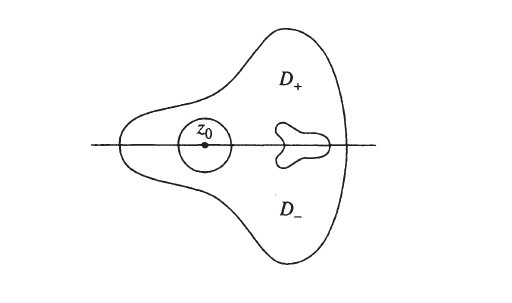
\includegraphics[width = 0.7 \textwidth]{schwarzov_princip_zrcaljenja.png}
    \end{center}
    \begin{proof}
        Dokaz temelji na uporabi karakterizacije harmoničnih funkcij s pomočjo lastnosti povprečne vrednosti, oziroma uporabi le-tega, za dokaz harmoničnosti eksplicitno podane razširitve, za katero trdimo, da je harmonična $D$.
    \end{proof}

\begin{thebibliography}{9}

\end{thebibliography}
\end{document}